\section{Optical Properties of the Sphere }
\label{sec:opt}


The central component of the experiment is the HPFS sphere, which holds the LXe target, located in the center of the detector system. In order to allowthe measurement of the original direction of photons emitted by the LXe, it is important to reduce the amount of diffractions and absorptions of photons on their path from the LXE to the PMTs.   

To insure the photones emitted by the LXe can be measured by the PMTs, the HPFS transparency to VUV photons is crucial parameter for setting the sphere's dimensions (inner and outer radii). 
Therefore, the transmittance of an HPFS sample was measured, using the above mention VUV monochromator. The deuterium light source\footnote{McPherson 632} spectrum is in the range of (110-190)\,nm, peaked at 160\.nm was facing a vacuum space. Using a PMT placed in the vacuum, the intensity of the light is measured, both with and without the HPFS sample. The ratio of the measured intensities is converted to the transmittance of the HPFS. The transmittances as a function of wavelength are shown in Fig.~\ref{fig:hpfsRIcalibration}~(right panel). The transmittance of the sample at 178~\,nm, is$\sim98.7$\,\%/cm.  

In order to reduce the diffraction in the LXe-HPFS transition, the sphere material is chosen to be HPFS, as he refractive index of it HPFS is 1.58 at 185 nm, matching to the LXe one, which is 1.61. The refractive index of this HPFS is 1.58 at 185 nm, matching to the LXe one, which is 1.61. The refractive index at various wavelengths was measured in Prof. Amos Breskin's lab using a VUV monochromator\footnote{McPherson 234/302VM}. The results of this measurements are shown in Fig.~\ref{fig:hpfsRIcalibration} (left panel). The sphere is made of two HPFS hemispheres bonded together.

\begin{figure}[h]
   \centering
   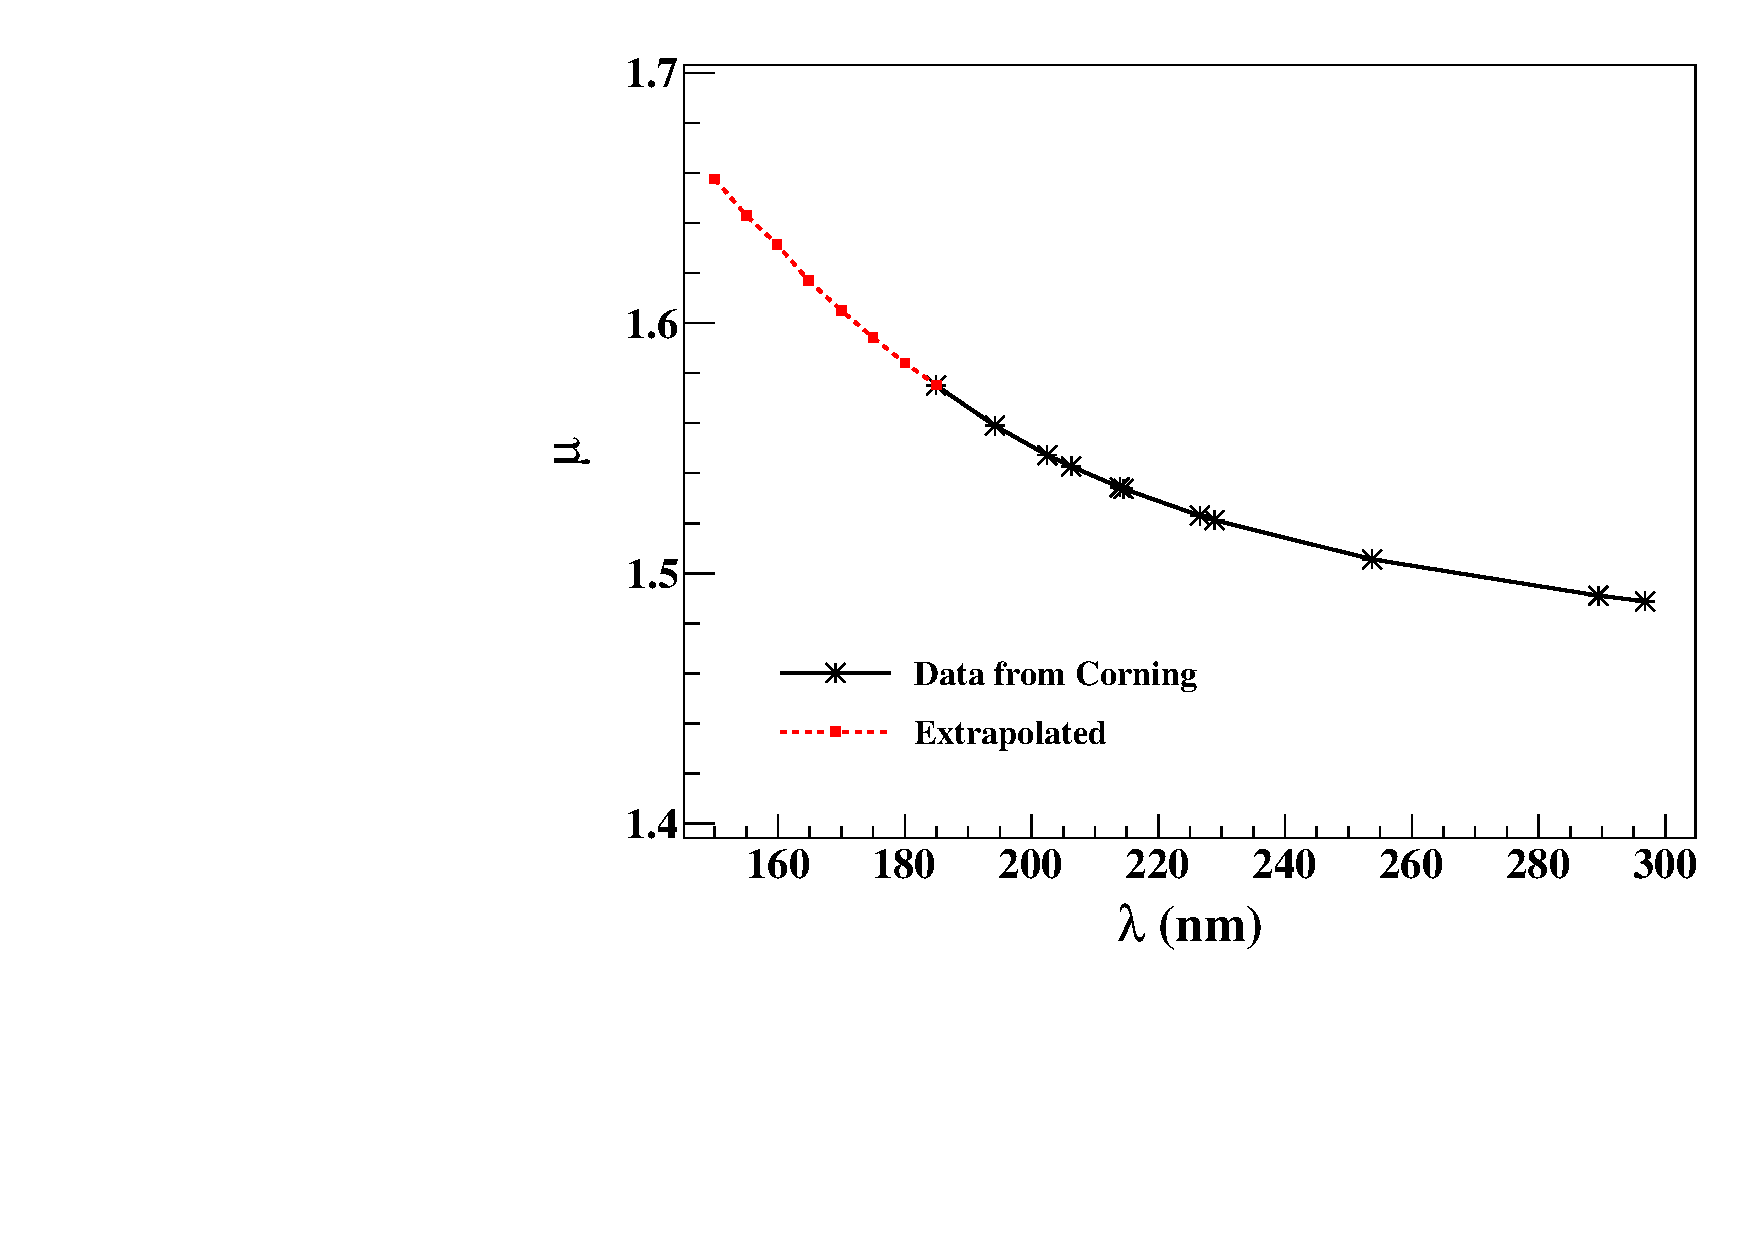
\includegraphics[width=0.48\textwidth]{RI-calibration.pdf}
    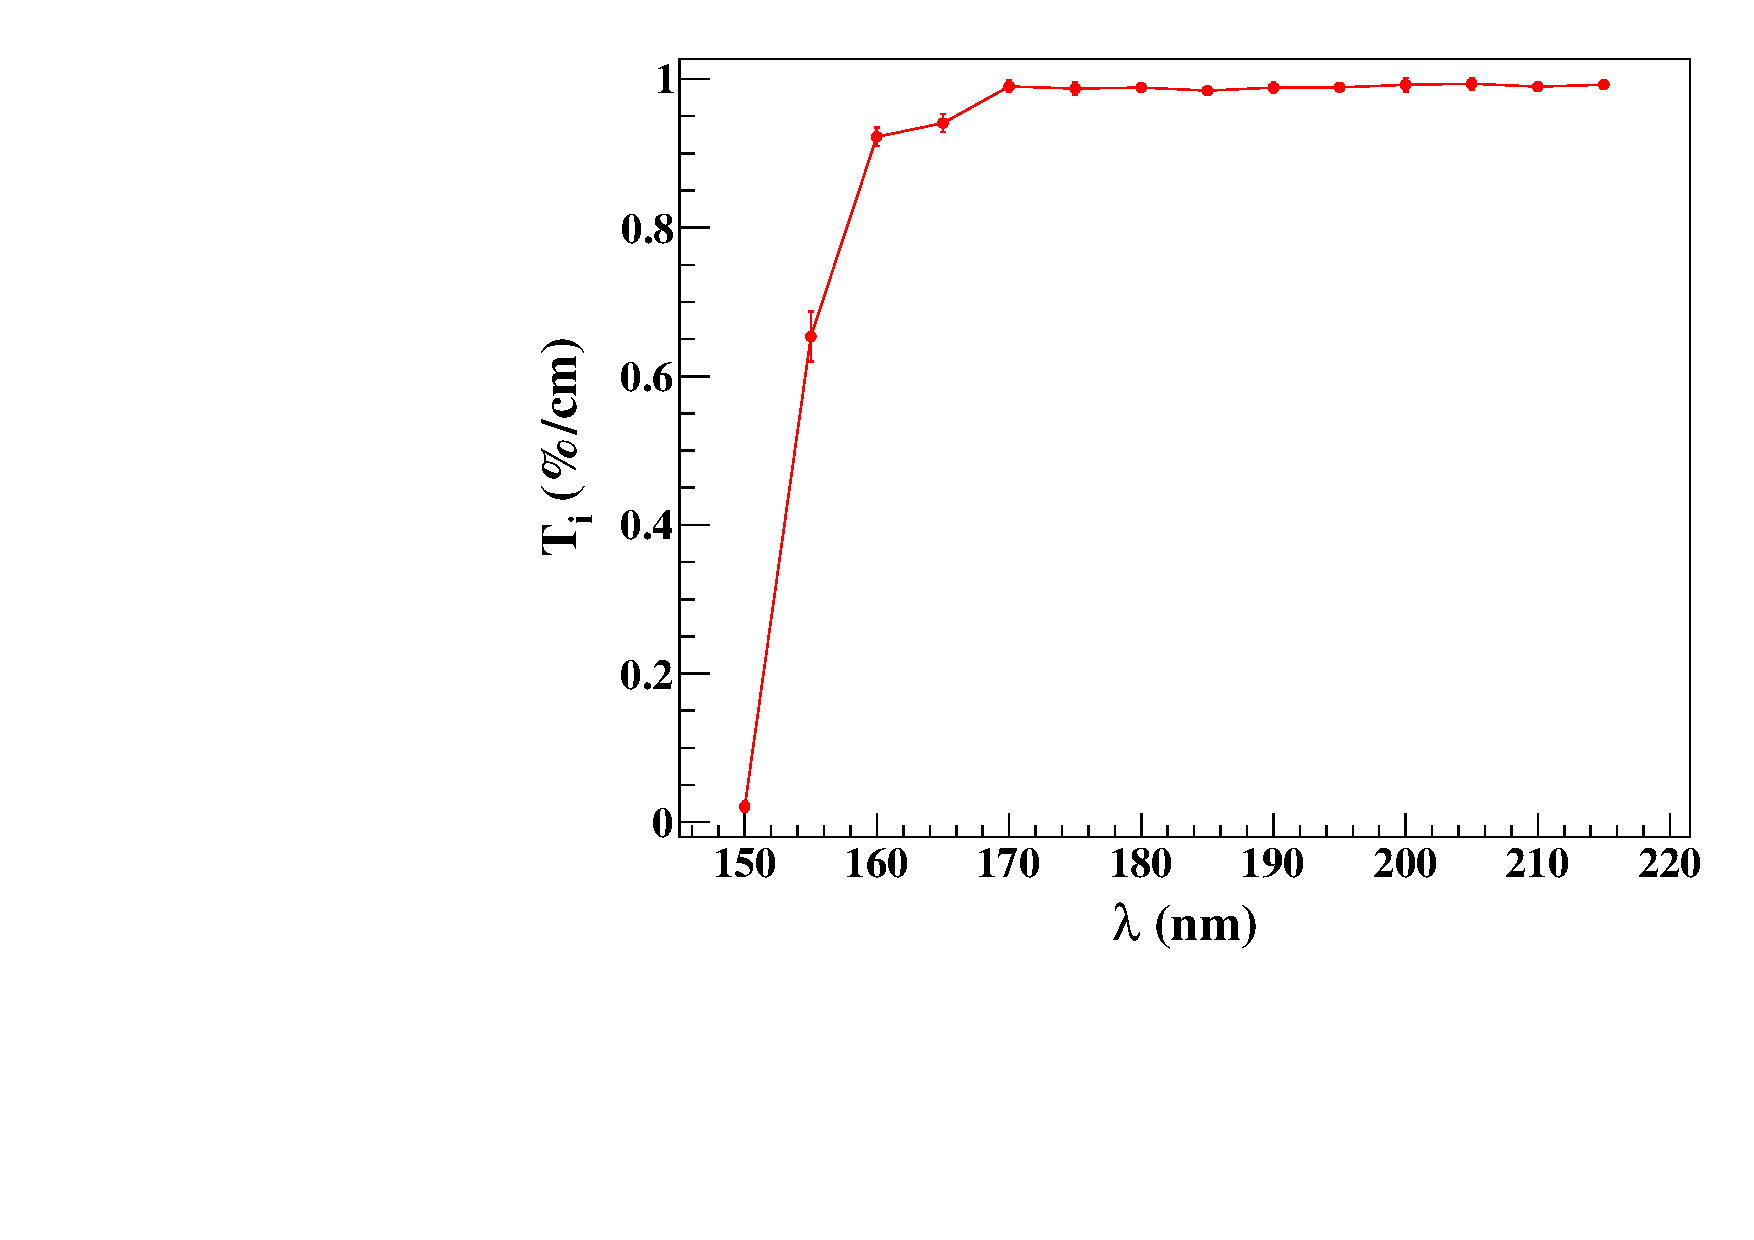
\includegraphics[width=0.48\textwidth]{IntTransmittance.pdf}
   \caption{Some relevant characteristics of HPFS-8655. (Left) The refractive index as provided by corning and 
   extrapolated to relevant wavelength range. (Right) The measured internal transmittance ($T_{i}$), the mean and RMS obtained from 10 sets of 
measurements are shown.}  
   \label{fig:hpfsRIcalibration}
\end{figure}


Finally, in oder to reduce the diffraction in the HPFS-Vacuum transition as well as internal reflections, the sphere should be thick so all photons will arrive in a perpendicular angle to the HPFS surface. In addition the sphere must not be too thick not to attenuate the scintillation light. The LXe target bubble within should be large to increase the detector medium but not be too large in order to avoid double scatters. Using a GEANT4 based simulation~\cite{AGOSTINELLI2003250} studying the path of the scintillation photons the sphere dimensions are optimized. The outer radius is chosen to be 3 cm, and the inner (the hollow space that holds the LXe) is chosen to be 1 cm. 


The sources that will be used for exciting the xenon and creating the supperradiance (signal) as well as the standard emission (background), will be $^{137} \mathrm{Cs}$ 
(E$_\gamma$=662 keV) and $^{57} \mathrm{Co}$ (E$_\gamma$= 122keV \& 136 keV) for ER with mean free path of $\sim4$\,cm and $\sim1$\,cm respectively. For NR, $^{241}$AmBe , D-D neutron generator, or neutron produced in an accelerator will be used. 



